\documentclass{standalone}
\usepackage{circuitikz}
\usepackage{schemabloc}

\newcommand{\sbEntreeT}[1]{
    \node [coordinate, name=#1] {};
    \sbDecaleNoeudx[0]{#1}{#1}
    \sbDecaleNoeudy[6]{#1}{#1}
}

\begin{document}
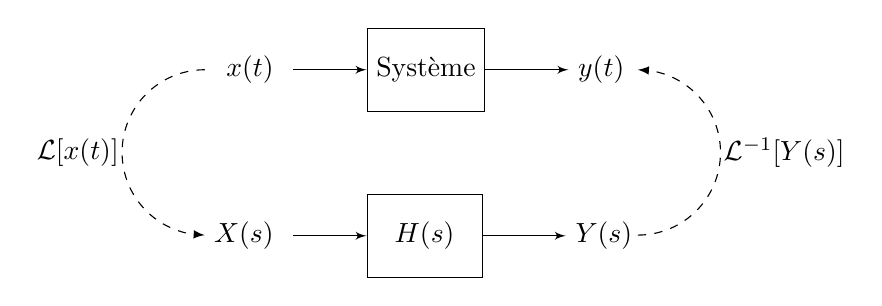
\begin{tikzpicture}
\sbEntree{X}
\sbBloc[3]{sys}{Système}{X}
\sbRelier{X}{sys}
\sbSortie[3]{Y}{sys}
\sbRelier{sys}{Y}
\node[left] at (X) {$x(t)$};
\node[right] at (Y) {$y(t)$};


\sbEntreeT{Xs}
\sbBloc[3]{sys_s}{~~$H(s)~~$}{Xs}
\sbRelier{Xs}{sys_s}
\sbSortie[3]{Ys}{sys_s}
\sbRelier{sys_s}{Ys}
\node[left] at (Xs) {$X(s)$};
\node[right] at (Ys) {$Y(s)$};

\draw[->, >=latex, dashed] (-1,0) arc[start angle=90, end angle=270, radius=1.05] node[midway, xshift=-1.6em](){$\mathcal{L}[x(t)]$};
\draw[->, >=latex, dashed] (4.5,-2.1) arc[start angle=270, end angle=450, radius=1.05] node[midway, xshift=2.3em](){$\mathcal{L}^{-1}[Y(s)]$};
\end{tikzpicture}
\end{document}